\chapter{The Impossibility of Early Violation Detection}
\label{chapter:finite-satisfiability}

In this chapter,
we show that it is undecidable whether or not a given set of rules is finitely satisfiable,
i.e.,
whether or not there is a finite instance that satisfies it.
This result
indicates that early violation detection
is impossible in general.
Combined with Chapters\:\ref{chapter:early-violation-detection}
and \ref{chapter:aggregation},
this indicates
that acyclicity for a set of rules forms a tight boundary
for solving early violation detection.

The chapter is organized as follows:
Section\:\ref{section:finite-satisfiability-definitions}
defines finite satisfiability
and states the main result.
Section\:\ref{section:finite-satisfiability-undecidable}
introduces a rule language Datalog$^{+}$ for technical development
and reduces the empty-tape halting problem for Turing machines
to the finite satisfiability of Datalog$^{+}$.
In Sections\:\ref{section:reduce-to-rules},
and \:\ref{section:finite-satisfiability-undecidable},
we show that finite satisfiability for a set of Datalog$^{+}$ rules
reduces to finite satisfiability for a set of rules,
completing the proof of the main result.
Finally,
in Sections\:\ref{section:finite-satisfiability-related-work} and \ref{section:finite-satisfiability-conclusion}
discuss related work and conclude the chapter.

\begin{figure}
    \centering
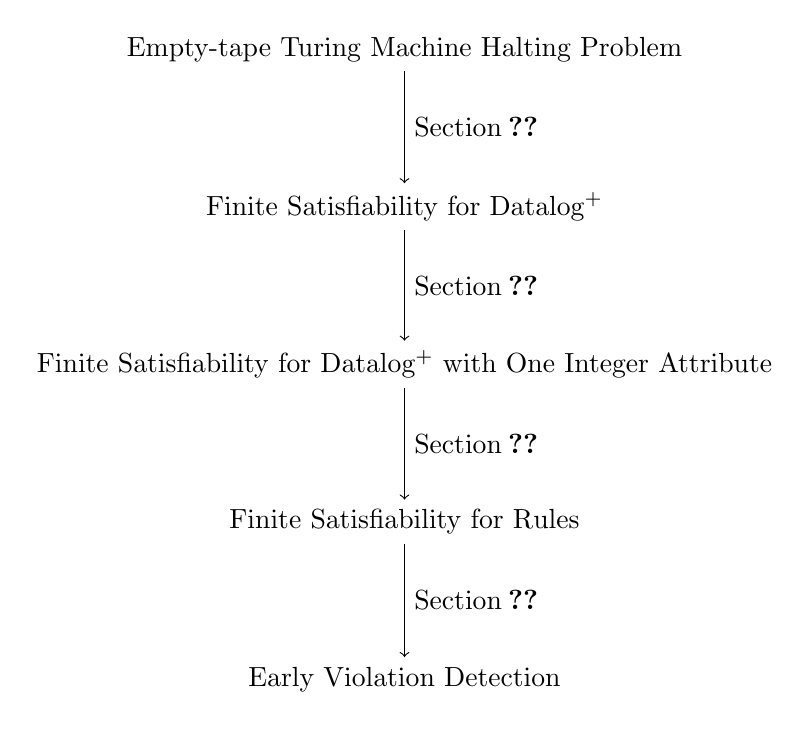
\begin{tikzpicture}[node distance = 2.0cm]
    \node[rectangle] (fin0) {Empty-tape Turing Machine Halting Problem};
    \node[rectangle, below of=fin0] (fin1) {Finite Satisfiability for Datalog$^{+}$};
    \node[rectangle, below of=fin1] (fin2) {Finite Satisfiability for Datalog$^{+}$ with One Integer Attribute};
    \node[rectangle, below of=fin2] (fin3) {Finite Satisfiability for Rules};
    \node[rectangle, below of=fin3] (fin4) {Early Violation Detection};
    \draw[->] (fin0) to node[right] {Section\:\ref{section:finite-satisfiability-undecidable}} (fin1);
    \draw[->] (fin1) to node[right] {Section\:\ref{section:two-attr}} (fin2);
    \draw[->] (fin2) to node[right] {Section\:\ref{section:reduce-to-rules}} (fin3);
    \draw[->] (fin3) to node[right] {Section\:\ref{section:finite-satisfiability-definitions}} (fin4);
\end{tikzpicture}
\caption{Structure of reductions}
\vspace{1cm}
\label{fig:reduction}
\end{figure}

\section{Early Violation Detection Solves Finite Satisfiability}
\label{section:finite-satisfiability-definitions}

In this section, we present the chapter's main result.
We first give the necessary definitions
for instances and finite satisfiability.
We then state the main theorem
and outline its proof.
Finally, we present
a corollary related to early violation detection.

Because we are interested in finite satisfiability of a set of rules,
rather than the online early violation detection problem,
we do not use enactments as the objects of rule satisfaction;
instead, we say a set of rules is satisfied by an ``instance''.
For a set $S$ of event types,
an {\em instance} of $S$
is a mapping from each event type $T$ in $S$ to
a possibly-infinite set of events of type $T$.
For an instance $I$ and an event type $E$,
the {\em table} $I.E$ is the set of events,
also called {\em tuples},
of type $E$ in $I$.
An instance {\em satisfies} a rule or set of rules
with the same semantics
as satisfaction
for enactments
in Chapter\:\ref{chapter:preliminaries}.
A set of rules is {\it finitely satisfiable}
if there is a finite instance
that satisfies each rule in the set.
The {\em finite satisfiability problem} is to decide
whether a given set of rules is finitely satisfiable.

% \begin{examp}
% \label{example:not-finitely-satisfiable}
% Consider the rule: $r_0: \Request(u)@x$, $\Approve(v)@x+1$, $u \neq v$ $\rightarrow$ $\Request(v,z)$.
% Despite the cycle formed by the {\tt Request} atoms,
% the set $\{r_0\}$ is finitely satisfiable
% with the empty instance,
% or the instance
% $I_0=\{ \Request \mapsto \{\Request(\mbox{\em Alice})@1$, $\Request(\mbox{\em Bob})@2\}$,
% $\Approve \mapsto \{\Approve(\mbox{\em Bob})@2\} \}$.
% because the only assignment for $I_0$
% that satisfies the rule body
% $\{u \mapsto \mbox{\em Alice}, x \mapsto 1, v \mapsto \mbox{\em Bob}\}$,
% satisfies the rule head
% when extended with $z=3$.
% \end{examp}

\begin{figure}[h!]
    \centering
\begin{tabular}{|lcl|}
\hline
$r_1$ &:& $\true \rightarrow \Request(\mbox{\em Alice})@x$\\
$r_2$ &:& $\Request(u)@y \rightarrow \Approve(u)@y{+}1$\\
$r_3$ &:& $\Approve(v)@y \rightarrow \Request(v)@y{+}1$\\
\hline
\end{tabular}
    \caption{Set of rules that is not finitely satisfiable}
    \label{fig:unsat-constraint-rules}
\end{figure}

\begin{examp}\label{example:not-finitely-satisfiable}
Not every set of rules is finitely satisfiable;
consider the set of rules in Fig\:\ref{fig:unsat-constraint-rules}.
Let $I$ be an arbitrary instance satisfying
$\{r_1, r_2, r_3\}$.
Because $r_1$ has no atoms in the body,
$I$ must contain the event
$\Request(\mbox{\em Alice}, x)$
for some $x\in \mathbb{N}$;
without loss of generality,
we assume $x=1$.
Then, satisfying $r_1$ requires $I$ contain
$\Request(\mbox{\em Alice}, 1)$.
Applying $r_2$ to $\Request(\mbox{\em Alice}, 1)$,
$I$ contains $\Approve(\mbox{\em Alice}, 2)$.
Applying $r_3$ to $\Approve(\mbox{\em Alice}, 2)$,
$I$ contains $\Request(\mbox{\em Alice}, 3)$.
Then, applying $r_2$ to $\Request(\mbox{\em Alice}, 3)$
indicates $I$ contains $\Approve(\mbox{\em Alice}, 4)$.
Continuing in this manner,
$I$ contains $\Request(\mbox{\em Alice}, 2n+1)$
and $\Approve(\mbox{\em Alice}, 2n+2)$ for all $n\in \mathbb{N}$.
In summary,
the rule $r_1$ has no atoms in the body.
This forces the instance to contain
the event in the head of $r_1$.
that comes from applying $r_2$ and $r_3$.
That event
initiates the infinite chain of events.
Thus, $I$ is infinite;
because $I$ is arbitrary,
this shows no finite instance
can satisfy $\{r_1, r_2, r_3\}$.
\end{examp}

Given these definitions,
we can now state the main result of this chapter
in Theorem\:~\ref{thm:undecidability}.

\begin{thm}\label{thm:undecidability}
Finite satisfiability for a set of rules is undecidable.
\end{thm}

The remainder of this chapter is devoted to proving this theorem.
We place this result
in the context of early violation detection.
% An enactment $\eta{=}\{e_1, e_2, \ldots\}$
% can be placed in the head of a rule $r_\eta\,: \true \rightarrow e_1, e_2, \ldots$,
% so that all instances satisfying $r_\eta$
% contain $\eta$.
% Given a set of rules $R$,
% the set
% $R \cup \{r_\eta\}$ is finitely satisfiable
% only if
% $\eta$ can be extended to a finite enactment that satisfies $R$.
Finite satisfiability for a set of rules
is a special case of early violation detection
in which the enactment is empty,
as the empty enactment should be reported 
as a violation
if and only if the set of rules is not finitely satisfiable.
Then,
an algorithm that decides if a violation exists
also decides finite satisfiability.
This leads to the following corollary
of Theorem\:\ref{thm:undecidability}.
    
\begin{corollary}\label{col:undecidability}
Early violation detection for a set of rules is impossible.
\end{corollary}

Our proof of Theorem\:\ref{thm:undecidability} is structured as follows:
in Section\:\ref{section:finite-satisfiability-undecidable},
we introduce a language called Datalog$^{+}$
and show that the empty-tape halting problem
reduces to finite satisfiability for a set of Datalog$^{+}$ rules.
Then,
in Section\:\ref{section:reduce-to-rules},
we show that there is a mapping between
Datalog$^{+}$ and rules
that extends the undecidability result
for Datalog$^{+}$
to finite satisfiability for rules.

\section{Datalog$^{+}$}
\label{section:finite-satisfiability-undecidable}

In this section, we give definitions
for the central notions of the reduction,
including
Datalog$^{+}$,
the model of Turing machines
and the empty-tape halting problem.
Then,
we construct a reduction from the empty-tape halting problem
to finite satisfiability for Datalog$^{+}$ rules.   

For the technical development in the proof of Theorem\:\ref{thm:undecidability},
we define a new rule language called Datalog$^{+}$.
Datalog$^{+}$ has the same syntax and semantics as our rule language,
except that it does not use the timestamp ``@'' syntax
and each event type may have 
an arbitrary number of integer attributes,
instead of only data attributes.
Timestamp attributes take values from $\mathbb{N}$,
with the standard ordering $<$, addition $+$, equality $=$, and non-equality $\neq$ predicates.
An example of the syntax of Datalog$^{+}$ is shown in Fig\:\ref{fig:datalog-plus-syntax}.

\begin{figure}[h!]
    \centering
\begin{tabular}{|lcl|}
\hline
$r_1$ &:& $\true \rightarrow \Request(\mbox{\em Alice},x)$\\
$r_2$ &:& $\Request(u,y) \rightarrow \Approve(u,y{+}1)$\\
$r_3$ &:& $\Approve(v,y) \rightarrow \Request(v,y{+}1)$\\
\hline
\end{tabular}
    \caption{Set of Datalog$^{+}$ rules that is not finitely satisfiable}
    \label{fig:datalog-plus-syntax}
\end{figure}

A set of Datalog$^{+}$ rules
is satisfied by an instance,
with the same notion of finite satisfiability,
as defined for a set of rules.
Given this definition,
we state the following theorem,
proven in the remainder of this section.

\begin{thm}\label{thm:undecidability-extended-Datalog}
Finite satisfiability for a set of Datalog$^{+}$ rules is undecidable.
\end{thm}

In Example~\ref{example:not-finitely-satisfiable},
the event in the head of $r_1$
can be thought of as the input to a computation
and
chasing the rules $r_2$ and $r_3$
as an algorithm for the computation.
In this view,
whether or not the computation halts
corresponds to whether or not
the set of events required to satisfy the set of rules
is finite or infinite.
This suggests that
the halting problem
for Turing machine
is reducible to the finite satisfiability problem
for Datalog$^{+}$.
To show this,
we present the Turing machine
as a formal model of computation,
then 
show how to encode a Turing machine
as a set of Datalog$^{+}$ rules
in a way that matches its halting behavior
to the finite satisfiability problem.

\subsection{Turing Machines and the Empty-Tape Halting Problem}

We use a standard definition of Turing machines
and their computations \cite{GJ79}.
A {\it deterministic Turing machine} $M$
is a 5-tuple ($\Sigma$, $Q$, $q_0$, $F$, $\delta$,)
where
\begin{enumerate}
    \item $\Sigma$ is a non-empty set of {\it tape symbols},
    one of which is the {\it blank symbol} $\blank$,
    \item $Q$ is a non-empty set of {\it states}, with $q_0 \in Q$ as the {\it starting state}
    and $F \subseteq Q$ as a set of {\it halting states}, and
    \item $\delta$ is a partial {\it transition function}
	from $Q \times \Sigma$ to $Q \times \Sigma \times \{ L, R, \mbox{\em stay} \}$.
\end{enumerate}

Note that no input alphabet is defined because we consider only
computations where the input is empty.
The behavior of a Turing machine
is characterized as a sequence of configurations of the machine,
snapshots of the machine's state and tape contents,
recorded between each transition.
For the Turing machine $M$,
a {\it configuration} of $M$ is a triple $(w, j, s)$ where
\begin{itemize}
    \item $w$ is the {\it tape contents}, a finite word in the language
    $(\Sigma-\{\blank\})^*$,
    \item $j$ is the position of the read-head,
    such that $1{\leq}j{\leq}|w|+1$,
    indicating that the machine's read-head is reading
    the $j$-th symbol from the left in the non-blank portion
    of the tape
    \item $s$ is the state of the machine, i.e., a state in $Q$
\end{itemize}
% During the execution of a Turing machine,
% the machine's configuration changes
% according to the transition function $\delta$.
% A sequence of configurations that satisfies certain conditions is a computation of $M$.

% A {\it computation} $S$ is a sequence of configurations such that
% \begin{itemize}
%     \item if $S$ is finite, then the last configuration in $S$ has a halting state, and 
%     \item for all consecutive configurations $S(i)$ and $S(i+1)$ in $S$
%     such that $S(i)=(w, j, s)$,
%     \begin{itemize}
%         \item $\delta(w[j],s)$, i.e., the next transition is defined by $M$'s transition function,
%         \item if $\delta(w[j],s)=(s',e,L)$, then $w[j]\neq \blank$ and $S(i+1)=(w[j\mapsto e], j{-}1, s')$
%         (the machine is not directly to the right of a blank symbol and the tape at index $j$ is updated to $e$ and the read-head moves one cell to the left),
%         \item if $\delta(w[j],s)=(s',e,R)$, then
%         \begin{itemize}
%             \item if $j=|w|$, then $S(i+1)=(w[j\mapsto e]\blank,j+1,s')$
%             (the tape grows to the right by one symbol)
%             \item otherwise, $S(i+1)=(w[j\mapsto e], j+1, s')$ 
%         \end{itemize}
%         \item if $\delta(w[j],s)=(s',e,\mbox{\em stay})$, then $S(i+1)=(w[j\mapsto e], j, s')$
%         (the tape is not modified and the read-head does not move)
%     \end{itemize}
% \end{itemize}

% where $w[j\mapsto e]$ is the word $w$ with the character
% at position $j$ replaced by the symbol $e$
% and $w\blank$ is the word $w$ concatenated with the $\blank$ symbol.
% A computation is {\it halting} if it is finite.
Given any configuration $C$,
the subsequent configuration is determined only
by $C$ and the machine's transition function,
which maps each pair of a state and a tape symbol
to a unique triple of a state, a tape symbol, and a direction.
This makes our class of Turing machines {\it deterministic}. 
This definition only allows the machine to replace blank symbols
with symbols from the tape alphabet to the right of the read-head's starting position,
i.e., in one direction.
This makes it a {\it one-way} Turing machine.

We consider only computations that start with
the {\it empty-tape configuration},
i.e., with one $\blank$ symbol on the tape,
the read-head at position $1$ on the tape reading the $\blank$ symbol,
and the machine in the start state $q_0$.
The {\it empty-tape halting problem} asks:
does a given deterministic one-way Turing machine
halt after beginning with the empty-tape configuration?
This problem is known to be undecidable \cite{banitt2010halting}.

\subsection{Constructing a Set of Datalog$^{+}$ Rules for the Empty-Tape Halting Problem}
\label{subsection:finite-satisfiability-encoding}

We now encode the empty-tape halting problem
for an arbitrary Turing machine
as a set of Datalog$^{+}$ rules.
The encoding is based on the idea
that a Turing machine computation is a sequence of configurations.
We represent each configuration as a block of rows in a table,
one block per configuration.
We use the following tables:
\begin{itemize}
    \item $\Config$ encodes each of $M$'s configurations,
    starting with the empty-tape configuration,
    \item $\Next$ helps link successive configuration blocks 
    in $\Config$, so that only successive configurations
    that are valid according to $M$'s transition function
    are allowed,
    \item $\Error$ captures other conditions
    that $\Config$ and $\Next$ must satisfy
    to represent a valid computation of $M$,
    such as each configuration only having one machine state,
    with rules that trigger non-finite satisfiability
    if the computation is invalid.
\end{itemize}

Because the $\Config$ table stores each configuration
in the empty-tape computation of $M$,
it has an infinite number of rows
if and only if the machine has an infinite computation
on the empty tape.
Additionally,
$M$ is deterministic,
so the instance of $\Config$, $\Next$, and $\Error$
that satisfies $\Rules(M)$
is unique given $M$. 
Then,
$\Rules(M)$ is finitely satisfiable
if and only if
$M$ has a halting computation
on the empty tape.

\begin{table}[!ht]
    \centering
    \begin{tabular}{|c|c|c|c|c|c}\cline{1-5}
        \multicolumn{5}{|c|}{Transition Relation} & \\ \cline{1-5}\cline{1-5}
        {\em read}    & {\em state} & {\em write} & {\em nextState} & {\em dir} &
        \multirow{6}{*}{\adjustbox{valign=t}{
            \begin{tikzpicture}[
                node distance = 1.0cm,
                state/.style = {circle, draw, minimum size=0.4cm},
                arrow/.style = {->, >=stealth, shorten >=1pt, semithick}
              ]
              % States
              \node[state] (q0) {$q_0$};
              \node[state, right=of q0] (q1) {$q_1$};
              \node[state, right=of q1] (q2) {$q_2$};
              \node[state, right=of q2] (q3) {$q_3$};
              \node[state, right=of q3] (q4) {$q_4$};
              % Transitions
              \draw[->] (q0) to[out=45, in=135] node[midway,above] {$\blank$/0, R} (q3);
              \draw[->] (q0) to[loop below] node[midway,below] {1/0, R} ();
              \draw[->] (q1) to[loop below] node[midway,below] {0/1, L} ();
              \draw[->] (q4) to[loop below] node[midway,below] {1/1, \mbox{\em stay}} ();
              \draw[->] (q2) to[out=45, in=135] node[midway,above] {0/1, \mbox{\em stay}} (q4);
              \draw[->] (q3) to[out=-135, in=-45] node[midway,below] {$\blank$/1, L} (q2);
              \draw[->] (q2) to[out=-135, in=-45] node[midway,below] {$\blank$/1, L} (q1);
              \draw[->] (q1) to[out=45, in=135] node[pos=0.15,above] {1/1, L} (q3);
            \end{tikzpicture}
        }}                                                  \\\cline{1-5}
        $\blank$      & $q_0$ & 0     & $q_3$     & R     &    \\\cline{1-5}
        0       & $q_1$ & 1     & $q_1$     & L     &   \\\cline{1-5}
        0       & $q_2$ & 1     & $q_4$     & \mbox{\em stay}  &  \\\cline{1-5}
        $\blank$      & $q_3$ & 1     & $q_2$     & L     &  \\\cline{1-5}
        ...     &       &       &           &       &  \\\cline{1-5}
    \end{tabular}
    \vspace{0.1in}
    \caption{Transitions for the Turing Machine $M$}
    \label{tab:example-transition-table}
\end{table}

\begin{examp}\label{ex:tm-rules}
Figure\:\ref{tab:example-transition-table} shows the transition relation
for a running example Turing machine $M$,
along with a finite state machine diagram for $M$.
In the transition relation for $M$,
the first row indicates that
when a $\blank$ symbol is read and the machine is in state $q_0$,
the following configuration is achieved by
writing a $0$ symbol to the tape,
changing the machine's state to $q_1$,
and moving the read-head one tape cell to the right.
The second row indicates that
when a $\blank$ symbol is read and the machine is in state $q_1$,
the machine writes a $1$ symbol to the tape,
maintains the state $q_1$,
and moves the read-head one tape cell to the left.
\end{examp}

The $\Config$ event type
holds the machine's tape contents and read-head position.
It uses three attributes:
{\em index}, {\em tape}, and {\em state}.
The {\em index} is an integer attribute is unique for each row
and organizes the configurations,
with blocks of rows with consecutive indices
encode an individual configurations.
Finally, {\em tape} is a data attribute to hold tape symbols,
and {\em state} is a data attribute to hold machine states.

\begin{figure}[!ht]
    \captionsetup[subfigure]{labelformat=empty}
    \centering
    \begin{subfloat}[][]
        \centering
        \begin{tabular}{|p{1cm}|p{1cm}|p{0.5cm}|p{1cm}|p{1cm}|p{1cm}|p{5cm}}
            \cline{1-2}\cline{4-6}
            \multicolumn{2}{|c|}{\Next} &  & \multicolumn{3}{|c|}{\Config} &                                           \\\cline{1-2}\cline{4-6}\cline{1-2}\cline{4-6}
            {\em index} & {\em next} & & {\em index} & {\em tape} & {\em state}  & \multirow{3}{*}{\adjustbox{valign=m}{
                \hspace{0.5cm} configuration $C_1$ 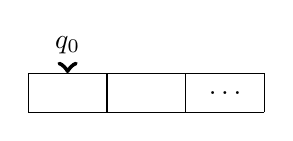
\begin{tikzpicture}
                    \draw (0,0) -- (3,0);
                    \draw (0,0.5) -- (3,0.5);
                    \draw (0,0) -- (0,0.5);
                    \node at (0.5,0.25) {$\blank$};
                    \draw (1,0) -- (1,0.5);
                    \node at (1.5,0.25) {$\blank$};
                    \draw (2,0) -- (2,0.5);
                    \node at (2.5,0.25) {$\dots$};
                    \draw (3,0) -- (3,0.5);
                    \draw[->,ultra thick] (0.5,0.55) -- (0.5,0.5);
                    \node at (0.5,0.85) {$q_0$};
                  \end{tikzpicture}
            }}                                                      \\\cline{1-2}\cline{4-6}\cline{1-2}\cline{4-6}
            0 & 2 & & 0       & \#        & \blank       &                \\\cline{1-2}\cline{4-6}
            1 & 3 & & 1       & \blank        & $q_0$   &                 \\\cline{1-2}\cline{4-6}\cline{1-2}\cline{4-6}
        \end{tabular}
    \end{subfloat}
    
    \begin{subfloat}[][]
        \centering
        \begin{tabular}{|p{1cm}|p{1cm}|p{0.5cm}|p{1cm}|p{1cm}|p{1cm}|p{5cm}}
            \cline{1-2}
            2 & 5 & & 2       & \#        & \blank       &  \multirow{2}{*}{\adjustbox{valign=m}{
                \hspace{0.5cm} configuration $C_2$ 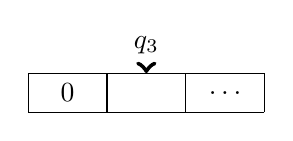
\begin{tikzpicture}
                    \draw (0,0) -- (3,0);
                    \draw (0,0.5) -- (3,0.5);
                    \draw (0,0) -- (0,0.5);
                    \node at (0.5,0.25) {$0$};
                    \draw (1,0) -- (1,0.5);
                    \node at (1.5,0.25) {$\blank$};
                    \draw (2,0) -- (2,0.5);
                    \node at (2.5,0.25) {$\dots$};
                    \draw (3,0) -- (3,0.5);
                    \draw[->,ultra thick] (1.5,0.55) -- (1.5,0.5);
                    \node at (1.5,0.85) {$q_3$};
                  \end{tikzpicture}
            }}                                          \\\cline{1-2}\cline{4-6}
            3 & 6 & & 3       & 0         & \blank       &    \\\cline{1-2}\cline{4-6}
            4 & 7 & & 4       & \blank        & $q_3$   &     \\\cline{1-2}\cline{4-6}
        \end{tabular}
    \end{subfloat}

    \begin{subfloat}[][]
        \centering
        \begin{tabular}{|p{1cm}|p{1cm}|p{0.5cm}|p{1cm}|p{1cm}|p{1cm}|p{5cm}}
            \cline{1-2}
            5 & 8 & & 5       & \#        & \blank       &  \multirow{3}{*}{\adjustbox{valign=t}{
                \hspace{0.5cm} configuration $C_3$ 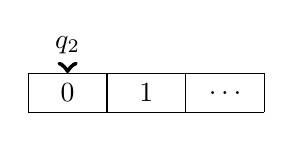
\begin{tikzpicture}
                    \draw (0,0) -- (3,0);
                    \draw (0,0.5) -- (3,0.5);
                    \draw (0,0) -- (0,0.5);
                    \node at (0.5,0.25) {$0$};
                    \draw (1,0) -- (1,0.5);
                    \node at (1.5,0.25) {$1$};
                    \draw (2,0) -- (2,0.5);
                    \node at (2.5,0.25) {$\dots$};
                    \draw (3,0) -- (3,0.5);
                    \draw[->,ultra thick] (0.5,0.55) -- (0.5,0.5);
                    \node at (0.5,0.85) {$q_2$};
                  \end{tikzpicture}
            }}                                      \\\cline{1-2}\cline{4-6}
            6 & 9 & & 6       & 0         & $q_2$   &     \\\cline{1-2}\cline{4-6}
            7 & 10 & & 7       & 1         & \blank  &     \\\cline{1-2}\cline{4-6}
        \end{tabular}
    \end{subfloat}

    \begin{subfloat}[][]
        \centering
        \begin{tabular}{|p{1cm}|p{1cm}|p{0.5cm}|p{1cm}|p{1cm}|p{1cm}|p{5cm}}
            \cline{1-2}
            8 & 11 & & 8       & \#        & \blank       &   \\\cline{1-2}\cline{4-6}
            $\dots$ & & & ...     &           &         &        \\\cline{1-2}\cline{4-6}
        \end{tabular}
    \end{subfloat}
    \caption{Four successive configurations of $M$ in the $\Config$ and {\Next} tables}
    \label{tab:example-config-table}
\end{figure}

\begin{examp}\label{ex:config-table}
Consider the Table \ref{tab:example-config-table},
the row with index $1$ represents the initial empty-tape configuration of a machine $M$,
shown as configuration $C_1$.
The {\em tape} column holds the tape's contents, initially the string $\blank$,
and the read-head position, $1$, and (starting) state $q_0$
is indicated by the row where the {\em state} column is not blank;
as $M$ is in state $q_0$ at the start of the computation.
The following configuration, $C_2$,
produced when $M$ writes $0$ to the tape, moves right, and changes from state $q_0$ to $q_3$,
is shown in the rows of $\Config$ with indices 3 and 4.
The rows with indices $6$ and $7$ represent the next configuration, $C_3$,
when $M$ writes $1$ to the tape, moves left, and changes
from state $q_3$ to $q_2$.
\end{examp}

The $\Next$ table indicates how consecutive configurations in a Turing machine computation
are arranged in the $\Config$ table.
An tuple $(i, j)$ in the $\Next$ table means information at index $i$ in $\Config$
is propagated to index $j$ in $\Config$ for the subsequent configuration, assuming one exists.
For the first three configurations shown in the $\Config$ table above,
the $\Next$ table is shown in Table \ref{tab:example-config-table}.
Note that the arithmetic difference between the two columns can grow,
because the length of the non-blank portion of the tape
grows by one from the first configuration to the second.

% \begin{table}[!ht]
%     \centering
%     \begin{tabular}{|c|c|}\hline
%         \multicolumn{2}{|c|}{\Next} \\\hline
%         {\em index}   & {\em next}    \\\hline\hline
%         0               & 2             \\\hline
%         1               & 3             \\\hline
%         2               & 5             \\\hline
%         3               & 6             \\\hline
%         4               & 7             \\\hline
%         5               & 8             \\\hline
%     \end{tabular}
%     \caption{The $\Next$ Table for the First Three Configurations}
%     \label{tab:example-next-table}
% \end{table}

The {\it initialization} rules
(Fig. \ref{fig:initialization-rules})
require that the {\Config} table has the initial empty-tape configuration,
i.e., a configuration with an empty tape and a read-head index of $1$,
and that the $\Next$ table indicates the indices
of the second configuration.
Because the body of these rules is vacuously true,
these tuples appear in all instances
that satisfy $\Rules(M)$.

\begin{figure}
    \centering
    \begin{tabular}{|lcl|}
        \hline
        \multicolumn{3}{|c|}{Initialization Rules}              \\\hline\hline
        $\true$ & $\rightarrow$ & \Config(0,\#,\blank)          \\\hline
        $\true$ & $\rightarrow$ & \Config(1,\blank,$q_0$)       \\\hline
        $\true$ & $\rightarrow$ & \Config(2,\#,\blank)          \\\hline
        $\true$ & $\rightarrow$ & \Next(0,1)                    \\\hline
        $\true$ & $\rightarrow$ & \Next(1,3)                    \\\hline
    \end{tabular}
\caption{The Initialization Rules for $M$}
\label{fig:initialization-rules}
\end{figure}

The following rules in $\Rules(M)$
encode the progression
the $\Config$ and $\Next$ tables
with respect to the machine's transition function.
These include ``normal'' transitions to the right or left,
where the machine's transition function is applied,
and ``extending'' transitions to the right,
when the machine advances into the blank portion of the tape
and the tape's length is extended by one.
Additionally, there is the ``stay'' rule,
which encodes the machine's transition function
when the machine does not move the read-head,
and the ``copy'' rule
shows how the $\Config$ and $\Next$ tables
map one configuration to the next.
Finally, they also include an ``error'' transition rule,
which triggers an error
if the machine transitions to the left
when the read-head is at the leftmost tape cell.

The {\it normal left transition} rule
encodes the leftward transition of the read-head.
For each of the machine's transitions
$\delta(a,s)=(b,s',L)$,
the machine changes state from $s$ to $s'$
when reading tape symbol $a$,
write a tape symbol $b$ to the tape cell below the read head,
and move the read head to the left.
This rule applies when the $\Next$ table
indicates that the row with index $x{-}1$ in $\Config$
corresponds to the row with index $y{-}1$ in $\Config$
in the machine's following configuration
and the row with index $x$ in $\Config$
has state $s$ and is reading tape symbol $a$.
The rule's head ensures that the row with index $y$ in $\Config$
has state $s'$ and writes tape symbol $b$
to the tape cell below the read head,
and the $\Next$ table is updated
with rows $\Next(x,y)$, $\Next(x+1,y+1)$, and $\Next(x+2,y+2)$.
The rule is:
\begin{align}
    \begin{split}
\Config(x{-}1,c,\blank), \Config(x,a,s), \Config(x+1,c',\blank),\\
\Next(x{-}1,y{-}1) \rightarrow \Config(y{-}1,c,\blank), \Config(y,b,\blank), \Config(y+1,c',s'),\\
\Next(x,y), \Next(x+1,y+1), \Next(x+2,y+2)
    \end{split}
\end{align}

The {\it normal right transition} rule
encodes the rightwards motion
of the read head when the read head is not on the rightmost cell of the tape,
using the same format as the left transition rule
for each transition $\delta(a,s)=(b,s',R)$,
\begin{align}
    \begin{split}
\Config(x{-}1,c,\blank), \Config(x,a,s), \Config(x+1,c',\blank),\\
\Next(x{-}1,y{-}1) \rightarrow \Config(y{-}1,c,\blank), \Config(y,b,\blank), \Config(y+1,c',s'),\\
\Next(x,y), \Next(x+1,y+1), \Next(x+2,y+2)
    \end{split}
\end{align}

The {\it extending right transition rule}
encodes the rightwards motion of the read head when the read head is on the rightmost cell of the tape. 
The machine performs a state change, writes a symbol to the tape cell below the read head, and moves the right, creating a new blank symbol in the read head's new position:
\begin{align}
    \begin{split}
\Config(x{-}1,c,\blank), \Config(x,a,s), \Config(x+1,\#,\blank),\\
\Next(x{-}1,y{-}1) \rightarrow \Config(y{-}1,c,\blank), \Config(y,b,\blank), \Config(y+1,\blank,s'),\\
\Config(y+2,\#,\blank), \Next(x,y), \Next(x+1,y+1), \Next(x+2,y+3)
    \end{split}
\end{align}

The {\it stay transition} rule
encodes the lack of movement of the read head for a stay transition,
which initiates a state change and writes a symbol to the tape cell below the read head, 
leaving the position
of the read head unchanged.
For each transition rule
$\delta(a,s)=(b,s',\mbox{\em stay})$,
the rule is:
\begin{align}
    \begin{split}
\Config(x{-}1,c,\blank), \Config(x,a,s), \Config(x+1,c',\blank),\\
\Next(x{-}1,y{-}1) \rightarrow \Config(y{-}1,c,\blank), \Config(y,b,s'), \Config(y+1,c',\blank),\\
\Next(x,y), \Next(x+1,y+1), \Next(x+2,y+2)
    \end{split}
\end{align}

The {\it copy} rule
prompts non-halting configurations in $\Config$ table to be copied into higher indices according to the $\Next$ table:
\begin{align}
    \begin{split}
\Config(x{-}1,c',\blank), \Config(x,c,\blank), \Config(x+1,c'',\blank), \Next(x,y)\\
\rightarrow \Config(y,c,\blank), \Next(x+1,y+1)
    \end{split}
\end{align}

Finally, $\Error$ rules in $\Rules(M)$
indicate when the tables fail
to represent a halting computation of $M$.
This may be because the instance 
does not obey the transition function or the initial configuration,
or because the $\Config$ or $\Next$ tables have inconsistent data.
The $\Error$ event type has a single attribute
and is ``thrown'' when an inconsistency is detected
by creating a tuple in the $\Error$ table,
which is then propagated by the {\it propagate error} rule.
to fill the $\Error$ table with an infinite number of tuples:
\begin{align}
\Error(x) \rightarrow \Error(x+1)
\end{align}

The {\it erring left transition} rule
encodes the impossibility
of the read-head moving left when the read head
is on the leftmost cell of the tape.
Attempting to move to the left indicates the Turing machine
is not performing a (valid) computation and inserts a row into the $\Error$ table,
which is then propagated infinitely:
\begin{align}
\Config(x{-}1,\#,\blank), \Config(x,a,s), \Next(x{-}1,y{-}1) \rightarrow \Error(0)
\end{align}

The {\it same index, different symbols error} rule
prevents one index in the $\Config$ table from
being mapped to two distinct tape symbols.
Each index corresponds to one tape cell
in one configuration of a machine,
thus the tape symbol must be unique.
For each pair of unique tape symbols $a$ and $b$ 
in the machine's tape alphabet,
we have the rule:
\begin{align}
\Config(x,a,s), \Config(x,b,s') \rightarrow \Error(0)
\end{align}

The {\it same index, different states} rule
enforces that each index $x$ in the $\Config$ table
is mapped to at most one state.
For each pair of unique states $s$ and $s'$,
we have the rule:
\begin{align}
\Config(x,a,s), \Config(x,b,s') \rightarrow \Error(0)
\end{align}

In summary,
given an arbitrary Turing machine $M$,
the set $\Rules(M)$ includes:
\begin{enumerate}
    \item The {\it initialization} rules, and
    \item Rules $6.1$ through $6.4$ for each of the machine's $\delta$ transitions,
    \item Rules $6.5$ through $6.9$
\end{enumerate}

\subsection{The Construction is a Reduction}
\label{subsection:reduction-sound-complete}

We now prove that
$\Rules(M)$ is finitely satisfiable
if and only if
$M$ has a halting computation on the initial empty-tape.
We first prove the forward direction,
that if $M$ has a halting computation on the initial empty-tape,
then $\Rules(M)$ is finitely satisfiable.
Then, we prove the reverse direction.

{\sl Claim A:}
If $M$ has a halting computation on the initial empty-tape,
$\Rules(M)$ is finitely satisfiable.

\begin{proof}
Assume $M$ has a halting computation on the empty-tape.
Then,
there is a finite computation $S$ of $M$ such that
$S(0)$ is the initial blank-tape configuration and
the last configuration of $S$ has a halting state.
We construct an instance $db(S)$
with event types
$\Config$, $\Next$, and $\Error$.

For each configuration $S(i)$ in $S$, 
we include tuples in $db(S).\Config$ and $db(S).\Next$ 
using the following mapping from configurations to tuples:

Let $db(S).\Config$ include the tuples in Table \ref{tab:initial-dbS-Config} to represent $S(0)$.

\begin{table}[!ht]
    \centering
    \begin{tabular}{|c|c|c|}
        \multicolumn{3}{c}{\bf db(S).\Config} \\\hline
        index   & tape    & state     \\\hline\hline
        0       & \#        & \blank         \\\hline  
        1       & \blank        & $q_0$     \\\hline  
        2       & \#        & \blank        \\ \hline  
    \end{tabular}
    \caption{Tuples in $db(S).\Config$ From Initial Configuration}
    \label{tab:initial-dbS-Config}
\end{table}

Similarly, let $db(S).\Next$ include the tuples in Table \ref{tab:initial-dbS-Next}
to represent the transition from $S(0)$ to $S(1)$.

\begin{table}[!ht]
    \centering
    \begin{tabular}{|c|c|}
        \multicolumn{2}{c}{\bf db(S).\Next} \\\hline
        index & next      \\\hline\hline
        0       & 2         \\\hline
        1       & 3         \\\hline
    \end{tabular}
    \caption{Tuples in $db(S).\Next$ From Initial Configuration}
    \label{tab:initial-dbS-Next}
\end{table}

Let $S(i).tape[j]$ be the symbol on the $j^{th}$ position of the tape in $S(i)$.
Let $|S(i)|$ be the length of the non-blank portion of the tape in the configuration $S(i)$.
If $S(i)$ is mapped to the tuples in Tables \ref{tab:construction_tuples_config_Si} and \ref{tab:construction_tuples_next_Si}
and these tuples are included in $db(S)$,
then $S(i+1)$ (if it exists) is mapped to the tuples
in Tables\:\ref{tab:construction_tuples_config_Si1} and \ref{tab:construction_tuples_next_Si1}
and those tuples are included in $db(S)$.

\begin{table}[!ht]
    \centering
    \begin{tabular}{|c|c|c|}
        \multicolumn{3}{c}{\bf db(S).\Config} \\\hline
        index   & tape            & state     \\\hline\hline
        $j$     & \#                & \blank    \\\hline  
        $j+1$   & $S(i).tape[1]$    & $q_0$     \\\hline  
        $j+2$   & $S(i).tape[2]$    & $q_0$     \\\hline  
        ...     & ...               & ...       \\\hline
        $j+|S(i)|+|S(i+1)|+1$ & \# & \blank     \\\hline  
    \end{tabular}
    \caption{Tuples in $db(S).\Config$ from $S(i)$}
    \label{tab:construction_tuples_config_Si}
    \quad
    \begin{tabular}{|c|c|}
        \multicolumn{2}{c}{\bf db(S).\Next} \\\hline
        index         & next                  \\\hline\hline
        $j+|S(i)|+1$    & $j+|S(i)|+|S(i+1)|+2$ \\\hline
        $j+|S(i)|+2$    & $j+|S(i)|+|S(i+1)|+3$ \\\hline
        ...             & ...                   \\\hline
    \end{tabular}
    \caption{Tuples in $db(S).\Next$ from $S(i)$}
    \label{tab:construction_tuples_next_Si}
\end{table}

\begin{table}[!ht]
    \centering
    \begin{tabular}{|c|c|c|}
        \multicolumn{3}{c}{\bf db(S).\Config} \\\hline
        index                   & tape        & state \\\hline\hline
        $j+|S(i)|+1$            & \#            & \blank         \\\hline  
        $j+|S(i)|+2$            & $S(i+1).tape[1]$   & \blank         \\\hline  
        ...                     & ...           & ...       \\\hline
        $j+|S(i)|+|S(i+1)|+2$   & \#            & \blank         \\\hline
    \end{tabular}
    \caption{Tuples in $db(S).\Config$ from $S(i+1)$}
    \label{tab:construction_tuples_config_Si1}
    \quad
    \begin{tabular}{|c|c|}
        \multicolumn{2}{c}{\bf db(S).\Next} \\\hline
        index         & next                  \\\hline\hline
        $j+|S(i)|+1$    & $j+|S(i)|+|S(i+1)|+2$ \\\hline
        $j+|S(i)|+2$    & $j+|S(i)|+|S(i+1)|+3$ \\\hline
        ...             & ...                   \\\hline
        $j+|S(i)|+|S(i+1)|+2$ & $j{+}|S(i)|{+}|S(i{+}1)|{+}|S(i{+}2)|{+}3$\\
        & ($+4$ if $S(i{+}2)$ extends the tape)
        \\\hline
    \end{tabular}
    \caption{Tuples in $db(S).\Next$ from $S(i+1)$}
    \label{tab:construction_tuples_next_Si1}
\end{table}

\medskip

To see the instance $db(S)$ is finite,
consider the following:
the computation $S$ is halting,
so the number of configurations in $S$ is finite. 
Each configuration $S(i)$ is mapped to $|S(i)|+2$ tuples,
so the $db(S).\Config$ and $db(S).\Next$ tables
each have a finite number of tuples.
We do not add any tuples in $db(S).\Error$,
so $db(S).Error$ is empty by construction.
Each table in $db(S)$ is finite,
so $db(S)$ is finite.

\medskip

Now we show $db(S)$ satisfies $\Rules(M)$.
We do this by showing
$db(S)$ satisfies each rule in $\Rules(M)$.
The construction of $db(S)$ directly includes
the tuples required by the initial configuration rules
as the tuples mapped from $S(0)$.
For the normal transition left rule,
assume $db(S)$ satisfies the body of the rule 
with tuples
$\Next(x,y)$,
$\Config(x{-}1,c,\blank)$,
$\Config(x,a,s)$,
and
$\Config(x+1,c',\blank)$.

Because the indices in the $\Config$ events are consecutive,
they are created by some configuration $S(i)$ in $S$.
Because the transition rule requires that the state $s$ is not halting,
there is a configuration $S(i+1)$ following $S(i)$.
Because $S(i)$ and $S(i+1)$ obey the Turing machine's transition function,
$S(i+1)$ will have
symbol $c$ is at index $y{-}1$,
symbol $b$ at index $y$,
and symbol $c'$ at index $y+1$ on its tape,
and the read-head of the machine will be at index $y{-}1$ with state $s'$.
Additionally, $S(i)$ maps to a tuple in $\Config$ with index $x$
so in $db(s)$, $\Next$ contains the tuple $(x{-}1,y{-}1)$.
Then, $S(i+1)$ is mapped to the tuples
$\Config(y{-}1,c,s')$,
$\Config(y,b,\blank)$,
and $\Config(y+1,c',\blank)$,
as well as
$\Next(x+1,y+1)$,
$\Next(x,y)$,
and $\Next(x+2,y+2)$ in $db(S)$.
Then, $db(S)$ contain the tuples expected by the head
of the rule for the assumed tuples.

For the erring transition left rule:
Because $S$ is a valid computation in $M$,
there are no movements of the read-head to the left of the left end of the non-blank tape,
so tuples reflecting such a transition will not be inserted into $db(S)$.
Then, the body of this rule will never be triggered,
so this rule is vacuously satisfied.

For the normal transition right right,
the reasoning is identical to that of the normal transition left rule,
but with $\Config(y{-}1, c_1, \blank)$ and $\Config(y+1, c_2, s')$
instead of $\Config(y{-}1,c_1,s_2)$ and $\Config(y+1,c_2,\blank)$.
For the extending transition right rule,
the reasoning is identical to that of the normal transition right rule,
but with $\Next(x+1, y+2)$ and $\Next(x+2, y+3)$
instead of $\Next(x+1,y+1)$ and $\Next(x+2,y+2)$.
For the stay rule,
the reasoning
is identical to that of the normal transition right rule,
but with $\Config(y{-}1, c_1, \blank)$ and $\Config(y, b, s')$
instead of $\Config(y{-}1,c_1,\blank)$ and $\Config(y,b,\blank)$.

For the copy rule,
assume $db(S)$ satisfies the body of the copy rule with tuples
$\Next(x,y)$,
$\Config(x{-}1,c'',\blank)$,
$\Config(x,c,\blank)$,
and $\Config(x+1,c'',\blank)$.
Let $S(i)$ be the configuration in $S$ that maps to these tuples in $db(S)$.
If $S(i)$ creates the tuple in $db(S).\Config$ with $x$
and $db(S).\Next$ contains $(x{-}1,y{-}1)$,
then $(x, y)$ and $(x+1, y+1)$ are corresponding tape positions in $S(i)$ and $S(i+1)$.
Because $S(i)$ and $S(i+1)$ are consecutive configurations in $S$,
$c$ will appear at tape position $y$ in $S(i+1)$.
By construction, $db(S)$ will contain the tuples $\Config(y,c)$
and $\Next(x+1, y+1)$.
Then the tables $db(S).\Config$ and $db(S).\Next$ will contain the tuples expected by the rule for these tuples.

\medskip

Now we show the instance $db(S)$
satisfies the rules
regarding the $\Error$ table.
Because no tuple is added to the $\Error$ table
in the construction of $db(S)$,
the propagate error rule is vacuously satisfied.

For the erring transition left rule,
$S$ is a valid computation in $M$,
so there are no transitions to the left of the left end of the non-blank tape,
so the body of this rule is never triggered,
so this rule is vacuously satisfied.

For the same index, different symbols error rule,
In the construction of $db(S)$,
each index used in $db(S).\Config$
corresponds to one non-blank tape cell
in exactly one configuration in $S$ or to the left-end and respectively right-end blank tape cell in 
consecutive configurations in $S$.
Then, for each index in $db(S).\Config$
associated with a non-blank symbol,
there is exactly one tape cell that generates a tuple with that index,
so the tape symbol will be unique.
In the case that the index is associated with a blank symbol
from the left-end and right-end of the tape in consecutive configurations,
the tape symbol is the blank symbol,
so the tape symbol associated with the index is unique.

For the same index, different states error rule,
in the construction of $db(S)$,
each index used in $db(S).\Config$ corresponds to one non-blank tape cell
in exactly one configuration in $S$ or to the left-end and respectively right-end blank tape cell in 
consecutive configurations in $S$.
Then, for each index in $db(S).\Config$ associated with a state,
there is exactly one tape cell that generates a tuple with that index,
meaning the tape symbol will be unique.
In the case that the index is associated with a blank symbol
from the left-end and right-end of the tape in consecutive configurations,
the state symbol is the blank symbol,
so the state associated with the index is unique.

The above cases show that $db(S)$ satisfies every rule in $\Rules(M)$.
This,
along with the fact that $db(S)$ is finite,
shows there is a finite instance satisfying $\Rules(M)$.
This concludes the proof of the $\Leftarrow$ direction.
\end{proof}

Now we show if $\Rules(M)$ is finitely satisfiable,
then $M$ has a halting computation on the empty-tape.
We do this by constructing a computation $S$ in $M$
from a finite instance $I$ satisfying $\Rules(M)$.

{\sl Claim B:}
If $\Rules(M)$ is finitely satisfiable,
$M$ has a halting computation on the initial empty-tape.

\begin{proof}
Assume $\Rules(M)$ is finitely satisfiable.
Then, there is a finite instance $I$ that satisfies $\Rules(M)$.
Because $I$ satisfies $\Error(x) \rightarrow \Error(x+1)$
and $I$ is finite,
no {\em error} rules are not triggered by $I$.
Then,
the table $I.\Error$ is empty.
Then,
the {\it same index, different symbols}
and {\it same index, different states}
rules are not triggered by $I$.
Then,
every index in $I.\Config$ is paired with
at most one state and at most one tape symbol.

In the following,
we show $I$ encodes
a halting computation of $M$
by showing consecutive sets of tuples in $I$
correspond to consecutive configurations
in a computation in $M$.

Let $\tm$ be a mapping from sets of consecutive tuples in $I$
to configurations of $M$.
For each set of consecutive tuples in $I.\Config$
with indices $[i,i+k]$ such that indices $i{-}1$ and $i+k+1$ have $\#$ in the {\em tape} column
and
no other indices in $[i,i+k]$ have $\#$
in the {\em tape} column,
let $tm(i, i+k)$ be the configuration of $M$ such that
\begin{itemize}
\item the tape contents are the sequence of symbols in the {\em tape} column,
ordered by the indices
\item the read-head position is the position on the tape
(relative to $i$)
of the state symbol
that is not ``-'' in the state column
\item the machine state is the state symbol that is not ``-'' in the state column
\end{itemize}

Now we show that $I$ is a valid computation in $M$.
Let $tm(i, j)$ be a configuration of $M$
that does not have a halting state
and $I$ contain $\Next(i, j)$ and $\Next(i+1, j+1)$.
We show that for some $k\ge j$, $\tm(i, j)$ and $\tm(j, k)$ are consecutive configurations
in a computation of $M$ and
$I$ contains $\Next(j, k)$ and $\Next(j+1, k+1)$.
Let $i+w$ be the position of the machine's state in tuples with indices in the range $[i, j]$.
There are two cases of $i+w$.

{\bf Case 1}: $i+w=i+1$, i.e., the tuple in $I.\Config$ with index $i+1$ has a machine state. 
Because $\tm(i,j)$ is not halting,
there is a configuration of $M$ following $\tm(i, j)$.
Then, one of the transition rules applies with $x=i+1$ and
$I$ contains
$\Next(i+1, j+1)$,
$\Next(i+2, j+2)$, and
$\Next(i+3, j+3)$
(or $\Next(i+3, j+4)$ in the case that the extending right transition rule applies).
Then, the copy rule can be applied with index pairs $(x=i+3, y=j+3)$.
Then, the copy rule can be applied with index pairs $(x=i+4, y=j+4), \dots, (x=j{-}1, y=k)$
for some $k$ because if the copy rule applies with $i+2$,
the copy rule requires that $\Next(i+3,j+3)$ be present,
which will trigger the copy rule with $i+4$
unless a non-``-'' state appears.
In this case, the machine's state for $\tm(i,j)$ is at index $i+1$,
so the next non-``-'' state for not until at least $j+1$.
Then, the copy rule copes all tuples with indices in the range $[i+3, j]$ in $\Config$,
along with $\Next(j, k$) and $\Next(j+1, k+1)$ for some $k$.


{\bf Case 2}: $i+w>i+1$, i.e., the tuple in $I.\Config$ with index $i+1$ does not have a machine state.     
Then, the copy rule applies to tuples with $(x, y)$ values:
$(x=i+1, y=j+1), (x=i+2, y=j+2), ... (x=i+w-2, y=j+w-2)$,
because each time the copy rule applies with some $(x=a, y=b)$,
the copy rule requires the presence of $\Next(a+1,b+1)$.
This ensures the copy rule is triggered for the value $a+1$
unless a non-``-'' state appears in the tuple with index $a+2$.
In this case, the next non-``-' 'state is in the tuple with index $i+w$.
Then the $\Next$ table must have the row $\Next(i+w{-}1, j+w{-}1)$.
Because the tuple with index $i+w$ contains a state
and $I$ contains $\Next(i+w{-}1, j+w{-}1)$,
a transition rule can be applied.

There is a configuration of $M$ following $tm(i, j)$.
Then one of the transition rules is triggered with $x=i+w$,
ensuring the tuples with indices $i+w{-}1$, $i+w$, and $i+w+1$,
are mapped to the appropriate symbols and state
in tuples with indices $j+w+1$, $j+w+2$, and $j+w+3$ in $\Config$. 
Finally, applying the transition rule with $x=i+w$ requires the instance to have
$\Next(i+w, j+w)$ and $\Next(i+w+1, j+w+1)$,
and $\Next(i+w+2, j+w+2)$
(or $\Next(i+w+2, j+w+3)$,
if the extending right transition rule applies).
Then, the copy rule applies with $x=i+w+2$, $x=i+w+3$, $\dots, x=j+w{-}1$,
because when the copy rule applies with $x$,
the tuple $\Next(x+1,y+1)$ must be present,
ensuring that the copy rule is triggered with $x+1$ unless a non-``\blank'' state appears.
In this case, the first non-``-'' state is no earlier than the tuple in $\Config$ with index $j+w$.

\medskip

Given that $I$ encodes a computation of $M$,
we show that this computation is finite and halting. 
For sake of contradiction,
assume that $M$ does not have a halting computation on the empty-tape.
We show that this implies $I$ is infinite,
which contradicts the fact that $I$ is finite.

Because $M$ does not have a halting computation on the empty-tape,
there is an infinite monotonically increasing sequence $K$ of indices in $I.\Config$ such that $\tm(k(i), k(i+1))$ is a configuration in a computation of $M$ on the empty-tape and $I$ contains $\Next(k(i+1), k(i+2))$ and $\Next(k(i+1)+1, k(i+2)+1)$.
We prove this by strong induction on the index $i$.

Base Case: Let $k(1)=0$, $k(2)=2$. Because $I$ satisfies $\Rules(M)$, the $\Config$ table in $I$ satisfies the Initialization rule. Then, $tm(0,2)$ corresponds to the initial configuration to $M$ on the empty-tape and $I$ contains $\Next(0,2)$ and $\Next(1, 3)$.

Inductive Hypothesis: Assume there are some indices $k(i)$, $k(i+1)$ such that $tm(k(i)$, $k(i+1))$ is a configuration in a computation of $M$ on the empty-tape and $I$ contains $\Next(k(i+1), k(i+2))$ and $\Next(k(i+1)+1, k(i+2)+1)$.

With the assumption that $\tm(k(i), k(i+1))$ does not have a halting state, 
we know
there is some $k'$ such that $tm(k(i+1), k')$ follows $tm(k(i), k(i+1))$ and $I$ contains $\Next(k(i+1), k')$ and $\Next(k(i+1)+1, k'+1)$. 
Let $k(i+2) = k'$.
Then, $I$ has a tuple for each element of the infinite monotonically increasing sequence $K$,
so $I$ is infinite.
This contradicts the assumption that $I$ is finite.
Then,
we conclude $M$ has a halting computation on the empty-tape.
This concludes the proof of the $\Rightarrow$ direction.
\end{proof}

This concludes both directions of logical implication.
Theorem\:\ref{thm:undecidability-extended-Datalog}
follows from the undecidability of the empty-tape halting problem
\cite{banitt2010halting}
and this reduction from
the empty-tape halting problem
is reduced to the finite satisfiability problem for rules.
In the next section,
the encoding is shown to hold when
Datalog$^{+}$ is limited to only one integer attribute.

\section{Datalog$^{+}$ with One Integer Attribute}
\label{section:two-attr}

It is natural to ask whether the undecidability result
holds for events with one integer attribute,
as an increasing number of integer attributes
suggests an increase in the scale or complexity
of enactments and sets of rules.
In this section, we show that finite satisfiability
for Datalog$^{+}$ rules with
exactly one integer attribute
is undecidable,
by showing
all events in the encoding $\Rules(M)$
can be simulated with events
with one integer attribute.
Then, the proof of Theorem\:\ref{thm:undecidability}
holds with this restriction.

\begin{thm}\label{thm:two-attr}
Finite satisfiability for a set of Datalog$^{+}$ rules
with one integer attribute is undecidable.
\end{thm}

\begin{proof}
Given Theorem\:\ref{thm:undecidability-extended-Datalog},
it is sufficient to show
Theorem\:\ref{thm:two-attr}
by showing that
$\Config$, $\Next$, and $\Error$
can be simulated with event types with one integer attribute.
The simulation works as follows:
let $X(a_1,\dots,a_n)$ be an event types with $n$ attributes
Then, we can create $n$ new event types
$X_1$, $X_2$, $\dots$, $X_n$,
each with one integer attribute.
The integer attribute of $X_i$ is $a_i$;
note that a data attribute $a_i$ in $X$ can be simulated
by an integer attribute in $X_i$,
as the integers have the same cardinality as the data domain,
as well as the equality and non-equality predicates.
The second attribute of each $X_i$ is a new data attribute {\em join},
which is used to join the $X_i$'s to simulate the $X$ event type.
We show how each of the four event types in $\Rules(M)$
is simulated by this encoding.

Recall that the {\Config} event type has three attributes:
\mbox{\em index}, \mbox{\em tape}, and \mbox{\em state}.
Then, we can simulate {\Config} events using the following three event types
with the new attribute {\em join}:
$C_1$(\mbox{\em index}, \mbox{\em join}),
$C_2$(\mbox{\em tape}, \mbox{\em join}), and
$C_3$(\mbox{\em state}, \mbox{\em join}).
Then,
each event atom $\Config(x,t,s)$
in a rule in $\Rules(M)$
is replaced with
$C_1(x,i)$, $C_2(t,i)$, $C_3(s,i)$,
where $i$ is a fresh variable in each replacement
of a $\Config$ atom.
Similarly,
$\Next$(\mbox{\em index}, \mbox{\em next})
can be simulated with event types
$\Next_1$(\mbox{\em index}, \mbox{\em join}) and
$\Next_2$(\mbox{\em next}, \mbox{\em join}).
For rules with more than one $\Config$ or $\Next$ atom,
we use different variables $i_1,i_2,\dots$ for the {\em join} attribute
for each replacement
and include non-equality atoms between these join variables.
For example,
the copy rule:
\begin{align}
    \begin{split}
\Config(x{-}1,c',\blank), \Config(x,c,\blank), \Config(x+1,c'',\blank), \Next(x,y)\\
\rightarrow \Config(y,c,\blank), \Next(x+1,y+1)
    \end{split}
\end{align}
becomes
\begin{align}
    \begin{split}
\Config_1(x{-}1,i_1),   \Config_2(c',i_1),\Config_3(\blank,i_1),\\
\Config_1(x,i_2),       \Config_2(c,i_2),\Config_3(\blank,i_2),\\
\Config_1(x{+}1,i_3),   \Config_2(c'',i_3),\Config_3(\blank,i_3),\\
\Next_1(x,i_4), \Next_2(y,i_4)\\
\rightarrow
\Config_1(y,i_5), \Config_2(c,i_5),\Config_3(\blank,i_5),\\
\Next_1(x{+}1,i_6), \Next_2(y{+}1,i_6)
    \end{split}
\end{align}

Finally, note that the $\Error$ event type already
has one integer attribute and no data attributes,
so it is trivial to simulate.
% Additionally,
% for each new event type $E$({\em attr}, {\em join}),
% we add the rule $E(a, j), E(b, j), a\neq b \rightarrow \Error(0)$
% along with all instances of $E$ in the rules,
% to prevent reuse of the join variables,
% ensuring they are unique for each simulated tuple.

Given a Turing machine $M$,
we can construct a set of rules
using the new event types.

Because the new event types simulate
the original tuples in $\Rules(M)$,
the proof of Theorem\:\ref{thm:undecidability-extended-Datalog} applies.
\end{proof}

\section{Proof of Theorem \ref{thm:undecidability}}
\label{section:reduce-to-rules}

It remains to be shown that 
the undecidability of finite satisfiability for Datalog$^{+}$ 
indicates the same result for the original rule language,
completing the proof of Theorem\:\ref{thm:undecidability}.
The previous section proves undecidability for Datalog$^{+}$
with one integer attribute,
so it is sufficient to show that
there is a mapping from this language
to the original rule language
that preserves finite satisfiability.
We show this mapping exists
in Lemma\:~\ref{lemma:attribute-mapping}.

\begin{lemma}\label{lemma:attribute-mapping}
Let $R$ be a set of rules in Datalog$^{+}$
with one integer attribute.
There is a set $R'$ of constraints rule
that is finitely satisfiable
if and only if $R$ is finitely satisfiable.
\end{lemma}

\begin{proof}
Without loss of generality,
let $E(d_1, \dots, d_n, t)$
be an event type in $R$,
where $t$ is the integer attribute.
Note that this event type
generates events with exactly one timestamp.
Then,
there is an equivalent event type $E(d_1, \dots, d_n)$ for rules
as events for $E$ have a timestamp,
e.g., $E(\mbox{\em Alice})@10$,
and event atoms for $E$ have a timestamp variable,
e.g., $E(x, y, z)@t$.
Thus, $E(d_1,\dots,d_n,t)$ in Datalog$^{+}$
and $E(d_1,\dots,d_n)$ in rules
generate identical events
and have identical event atoms, modulo timestamp syntax.
Then,
to build $R'$,
replace each event atom $E(a_1,\dots,a_n,t)$ in $R$
with $E(a_1,\dots,a_n)@t$,
producing a rule
that is satisfied by the same instances as $R$.
Thus,
$R$ is finitely satisfiable if and only if $R'$ is finitely satisfiable.
\end{proof}

Then,
the undecidability of finite satisfiability for a set of Datalog$^{+}$ rules
with one integer attribute
implies the same result for a set of rules.

\section{Related Work}
\label{section:finite-satisfiability-related-work}

Finite satisfiability 
for first-order formulas,
a superclass of rules,
is undecidable,
which can also be proven by reduction
from the halting problem for empty-tape Turing machines \cite{libkin2004elements}.
A problem on
bounding the depth of recursion for Datalog programs
is also shown to be undecidable
by reduction from Turing machines \cite{hillebrand1995undecidable}.
Reference \cite{kolaitis2006complexity}
indicates undecidability of finite satisfiability
for source-to-target tuple-generating dependencies,
a class of formulas similar to rules
where a partition exists between event types
that appear in the body and event types 
that appear in the head.
Deciding finite satisfiability for rules is similar to
deciding 
the implication problem
for constrained tuple-generating dependencies,
for which chase techniques have been applied \cite{maher1996chasing, dou2013sound}.

\section{Chapter Summary}
\label{section:finite-satisfiability-conclusion}

In this chapter,
we showed that
the general problem of early violation detection
for a set of rules
is impossible,
given the undecidability of finite satisfiability.
It remains to be seen
if finite satisfiability for rules with additional restrictions,
such as using fewer data attributes,
is still unsolvable.
The chained encoding of the Turing machine tape
and successive potentially-infinite configurations suggests a similar reduction
with only unary event types is not possible.

